\scanpage{62}
\mspage{30}
la courbe modulaire $\widehat X^!_{0,4}$ sur $\widehat M^!_{0,4}$, avec ses quatre sections $s_0,s_1,s_\infty,s_\lambda$ (ou $t_1,t_2,t_3,t_4$) et avec l'opération de $\mathfrak S_4$ \deleted{dessus} sur $\widehat X^!_{0,4}\longrightarrow\widehat M^!_{0,4}$, échangeant ces quatre sections entre elles. Je vais pas le faire ici --- cela donnera du $=$ coup les \deleted{schémas}\inserted{multiplicités} modulaires $\widehat M_{0,4}$ et $\widehat X_{0,4}$. Pour $\widehat M_{0,4}$, il y a lieu de remplacer le diagramme (76) par un diagramme purement numérique
\[
(78)\quad\left\{\diagram{\begin{array}{c|c}
\text{codim }0&\text{codim }1\\\hline
\figure{\begin{tikzpicture}[baseline=-2pt]\fill (0,0) circle (1.4pt);\node[above] at (0,.15) {$4$};\end{tikzpicture}}\quad\xrightarrow{1}&
\figure{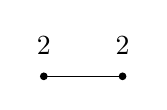
\begin{tikzpicture}[baseline=-2pt]\draw (0,0)--(1,0);\fill (0,0) circle (1.4pt);\fill (1,0) circle (1.4pt);\node[above] at (0,.15) {$2$};\node[above] at (1,.15) {$2$};\end{tikzpicture}}
\end{array}}\right.
\]
il n'y a plus qu'un seul pt à l'infini, correspondant aux trois pts à l'infini de $\widehat M^!_{0,4}$, permutés transitivement entre eux par $\mathfrak S_4$.

Caractéristiques d'EP fractionnaires. On trouve
\[
\begin{aligned}
\chi_!(M^{!\,\mathrm{an}}_{0,4})&=\chi_!(U^{\mathrm{an}}_{0,3})=2-2\underset{\substack{\Vert\\0}}{g}-\underset{\substack{\Vert\\3}}{\nu}=-1\\
\chi_!(\widehat M^{!\,\mathrm{an}}_{0,4})&=\chi_!(\mathbf P^{1\,\mathrm{an}})=2\\
\chi_!(\overset{\deleted{\unsure{\widehat{\phantom M}\,!}}}{M}{}^{\mathrm{an}}_{0,4})&=\chi_!(\unsure{U|\mathbf P}^{\mathrm{an}}_{0,3},\mathfrak S_4)\\
&=\chi_!\bigl(U^{\mathrm{an}}_{0,3}\smallsetminus\{\unsure{-\bar j},-j\}\smallsetminus\{\tfrac12,2,-1\},\mathfrak S_4\bigr)\\
&\qquad+\chi_!(\{\unsure{-\bar j},-j\},\mathfrak S_4)+\chi_!(\{\tfrac12,2,-1\},\mathfrak S_4)\\
&=-1+\frac13+\frac12=-\frac1{\unsure{24|6}}
\end{aligned}
\]
\margin{\uline{NB} On peut écrire directement $\chi_!(U^{\mathrm{an}}_{0,3}):[\mathfrak S_4]=-\frac1{24}$}
\margin{61}
